\documentclass{article}
\usepackage[utf8]{inputenc}
\usepackage[margin=1in]{geometry}
\usepackage{amsmath,amsfonts,amssymb}
\usepackage{graphicx}
\usepackage{hyperref}
\usepackage{float}
\usepackage{booktabs}
\usepackage{longtable}
\usepackage{algorithm}
\usepackage{algorithmic}
\usepackage{natbib}
\usepackage{url}
\usepackage{array}
\usepackage{xcolor}
\usepackage{multirow}
\usepackage{adjustbox}
\usepackage{siunitx}
\usepackage{makecell}
\usepackage{colortbl}
\usepackage{rotating}
\definecolor{bestgreen}{RGB}{0,150,0}
\definecolor{worstred}{RGB}{200,0,0}

\providecommand{\tightlist}{%
    \setlength{\itemsep}{0pt}\setlength{\parskip}{0pt}
}

% Fix any Unicode issues
\DeclareUnicodeCharacter{2212}{-}
\DeclareUnicodeCharacter{2264}{\leq}
\DeclareUnicodeCharacter{2265}{\geq}
\DeclareUnicodeCharacter{03B3}{\ensuremath{\gamma}}
\DeclareUnicodeCharacter{2080}{\ensuremath{_0}}
\DeclareUnicodeCharacter{2081}{\ensuremath{_1}}
\DeclareUnicodeCharacter{208A}{\ensuremath{_+}}
\DeclareUnicodeCharacter{2096}{\ensuremath{_k}}
\DeclareUnicodeCharacter{2207}{\ensuremath{\nabla}}
\DeclareUnicodeCharacter{03B5}{\ensuremath{\varepsilon}}
\DeclareUnicodeCharacter{2208}{\ensuremath{\in}}
\definecolor{bestgreen}{RGB}{0,150,0}
\definecolor{worstred}{RGB}{200,0,0}

\title{QQN: A Quadratic Hybridization of Quasi-Newton Methods for Nonlinear Optimization}
\author{Andrew Charneski\\SimiaCryptus Software}
\date{\today}

\begin{document}

    \maketitle

    \hypertarget{abstract}{%
\section{Abstract}\label{abstract}}

We present the Quadratic-Quasi-Newton (QQN) algorithm, a novel optimization method that combines gradient descent and quasi-Newton directions through quadratic interpolation.
QQN constructs a parametric path \(\mathbf{d}(t) = t(1-t)(-\nabla f) + t^2 \mathbf{d}_{\text{L-BFGS}}\) and performs univariate optimization along this path, creating an adaptive interpolation that requires no additional hyperparameters beyond those of its constituent methods.

We conducted comprehensive evaluation across 62 benchmark problems spanning convex, non-convex unimodal, highly multimodal, and machine learning optimization tasks, with 25 optimizer variants from five major families (QQN, L-BFGS, Trust Region, Gradient Descent, and Adam), totaling thousands of individual optimization runs.
Our results demonstrate that QQN variants achieve statistically significant dominance across the benchmark suite.
QQN algorithms won the majority of problems, with QQN-StrongWolfe showing particularly strong performance on ill-conditioned problems like Rosenbrock (100\% success rate) and QQN-GoldenSection achieving perfect success on multimodal problems like Rastrigin across all dimensions.
Statistical analysis using Welch's t-test with Bonferroni correction and Cohen's d effect sizes confirms QQN's superiority with practical significance.
While L-BFGS variants showed efficiency on well-conditioned convex problems and Adam-WeightDecay excelled on neural network tasks, QQN's consistent performance across problem types---requiring 50-80\% fewer function evaluations than traditional methods---establishes its practical utility as a robust general-purpose optimizer.

We provide theoretical convergence guarantees (global convergence under standard assumptions and local superlinear convergence) and introduce a comprehensive benchmarking framework for reproducible optimization research.
Code available at https://github.com/SimiaCryptus/qqn-optimizer/.

\textbf{Keywords:} optimization, quasi-Newton methods, L-BFGS, gradient descent, quadratic interpolation, benchmarking, statistical analysis

\hypertarget{paper-series-overview}{%
\subsection{Paper Series Overview}\label{paper-series-overview}}

This paper is the first in a planned series on optimization algorithms and their evaluation. It introduces:

\begin{enumerate}
\def\labelenumi{\arabic{enumi}.}
\tightlist
\item
  \textbf{A comprehensive optimizer evaluation framework} that will be used in subsequent papers to evaluate various optimization algorithms through rigorous statistical comparison.
\item
  \textbf{The Quadratic-Quasi-Newton (QQN) algorithm}, a new optimizer that combines gradient and quasi-Newton directions through quadratic interpolation.
\end{enumerate}

Planned subsequent papers in this series include:

\begin{itemize}
\tightlist
\item
  \textbf{QQN for Deep Learning}: Focusing on deep learning problems and simple QQN extensions such as adaptive gradient scaling (γ parameter) and momentum incorporation for handling the unique challenges of neural network optimization.
\item
  \textbf{Trust Region QQN}: Exploring how to constrain the quadratic search path using trust region methods for various specialized use cases, including constrained optimization and problems with expensive function evaluations.
\end{itemize}

This foundational paper establishes both the evaluation methodology and the core QQN algorithm that will be extended in future work.

\hypertarget{introduction}{%
\section{Introduction}\label{introduction}}

Optimization algorithm selection critically affects both solution quality and computational efficiency across machine learning, computational physics, engineering design, and quantitative finance.
Despite decades of theoretical development, practitioners face a fundamental trade-off between robustness and efficiency.
First-order gradient methods offer robust global convergence guarantees but suffer from slow linear convergence rates and poor performance on ill-conditioned problems.
Second-order quasi-Newton methods like L-BFGS achieve superlinear local convergence but can fail catastrophically with indefinite curvature, require complex line search procedures, and need careful hyperparameter tuning.
This tension intensifies in modern applications characterized by high dimensionality, heterogeneous curvature landscapes, severe ill-conditioning, and complex multimodal objective functions.

\hypertarget{previous-approaches-to-direction-combination}{%
\subsection{Previous Approaches to Direction Combination}\label{previous-approaches-to-direction-combination}}

Researchers have developed various approaches to combine gradient and quasi-Newton directions:

\begin{itemize}
\item
  \textbf{Trust Region Methods} \citep{conn2000trust}: These methods constrain the step size within a region where the quadratic model is trusted to approximate the objective function. While effective, they require solving a constrained optimization subproblem at each iteration.
\item
  \textbf{Line Search with Switching} \citep{morales2000automatic}: Some methods alternate between gradient and quasi-Newton directions based on heuristic criteria, but this can lead to discontinuous behavior and convergence issues.
\item
  \textbf{Weighted Combinations} \citep{biggs1973minimization}: Linear combinations of gradient and quasi-Newton directions have been explored, but selecting appropriate weights remains challenging and often problem-dependent.
\item
  \textbf{Adaptive Learning Rates} \citep{kingma2015adam}: Methods like Adam use adaptive learning rates based on gradient moments but don't directly incorporate second-order curvature information.
\end{itemize}

We propose quadratic interpolation as a simple geometric solution to this direction combination problem.
This approach provides several key advantages:

\begin{enumerate}
\def\labelenumi{\arabic{enumi}.}
\item
  \textbf{No Additional Hyperparameters}: While the constituent methods (L-BFGS and line search) retain their hyperparameters, QQN combines them in a principled way that introduces no additional tuning parameters.
\item
  \textbf{Guaranteed Descent}: The path construction ensures descent from any starting point, eliminating convergence failures common in quasi-Newton methods and providing robustness to poor curvature approximations.
  Descent is guaranteed by the initial tangent condition, which ensures that the path begins in the direction of steepest descent.
\item
  \textbf{Simplified Implementation}: By reducing the problem to one-dimensional optimization along a parametric curve, we leverage existing robust line-search methods while maintaining theoretical guarantees.
\end{enumerate}

\hypertarget{contributions}{%
\subsection{Contributions}\label{contributions}}

This paper makes three primary contributions:

\begin{enumerate}
\def\labelenumi{\arabic{enumi}.}
\item
  \textbf{The QQN Algorithm}: A novel optimization method that adaptively interpolates between gradient descent and L-BFGS through quadratic paths, achieving robust performance with minimal parameters.
\item
  \textbf{Rigorous Empirical Validation}: Comprehensive evaluation across 62 benchmark problems with statistical analysis, demonstrating QQN's superior robustness and practical utility.
\item
  \textbf{Benchmarking Framework}: A reusable Rust application for optimization algorithm evaluation that promotes reproducible research and meaningful comparisons.
\end{enumerate}

Optimal configurations remain problem-dependent, but QQN's adaptive nature minimizes the need for extensive hyperparameter tuning.
Scaling and convergence properties are theoretically justified, largely inherited from the choice of sub-strategies for the quasi-Newton estimator and the line search method.

\hypertarget{paper-organization}{%
\subsection{Paper Organization}\label{paper-organization}}

The next section reviews related work in optimization methods and benchmarking.
We then present the QQN algorithm derivation and theoretical properties.
Following that, we describe our benchmarking methodology.
We then present comprehensive experimental results.
The discussion section covers implications and future directions.
Finally, we conclude.

\hypertarget{related-work}{%
\section{Related Work}\label{related-work}}

\hypertarget{optimization-methods}{%
\subsection{Optimization Methods}\label{optimization-methods}}

\textbf{First-Order Methods}: Gradient descent \citep{cauchy1847methode} remains fundamental despite slow convergence on ill-conditioned problems.
Momentum methods \citep{polyak1964some} and accelerated variants \citep{nesterov1983method} improve convergence rates but still struggle with non-convex landscapes.
Adaptive methods like Adam \citep{kingma2015adam} have become popular in deep learning but require careful tuning and can converge to poor solutions.

\textbf{Quasi-Newton Methods}: BFGS \citep{broyden1970convergence, fletcher1970new, goldfarb1970family, shanno1970conditioning} approximates the Hessian using gradient information, achieving superlinear convergence near optima.
L-BFGS \citep{liu1989limited} reduces memory requirements to O(mn), making it practical for high dimensions.
However, these methods can fail on non-convex problems and require complex logic to handle edge cases like non-descent directions or indefinite curvature.

\textbf{Hybrid Approaches}: Trust region methods \citep{more1983computing} interpolate between gradient and Newton directions but require expensive subproblem solutions.
Unlike QQN's direct path optimization, trust region methods solve a constrained quadratic programming problem at each iteration, fundamentally differing in both computational approach and theoretical framework.
Switching strategies \citep{morales2000automatic} alternate between methods but can exhibit discontinuous behavior.
Our approach is motivated by practical optimization challenges encountered in production machine learning systems, where robustness often matters more than theoretical optimality.

\hypertarget{benchmarking-and-evaluation}{%
\subsection{Benchmarking and Evaluation}\label{benchmarking-and-evaluation}}

\textbf{Benchmark Suites}: \citet{dejong1975analysis} introduced systematic test functions, while \citet{jamil2013literature} cataloged 175 benchmarks.
The CEC competitions provide increasingly complex problems \citep{liang2013problem}.

\textbf{Evaluation Frameworks}: COCO \citep{hansen2016coco} established standards for optimization benchmarking including multiple runs and statistical analysis.
Recent work emphasizes reproducibility \citep{beiranvand2017best} and fair comparison \citep{schmidt2021descending}, though implementation quality and hyperparameter selection remain challenges.

\hypertarget{the-quadratic-quasi-newton-algorithm}{%
\section{The Quadratic-Quasi-Newton Algorithm}\label{the-quadratic-quasi-newton-algorithm}}

\hypertarget{motivation-and-intuition}{%
\subsection{Motivation and Intuition}\label{motivation-and-intuition}}

Consider the fundamental question: given gradient and quasi-Newton directions, how should we combine them?
Linear interpolation might seem natural, but it fails to guarantee descent properties.
Trust region methods solve expensive subproblems.
We propose a different approach: construct a smooth path that begins with the gradient direction and curves toward the quasi-Newton direction.

\hypertarget{algorithm-derivation}{%
\subsection{Algorithm Derivation}\label{algorithm-derivation}}

We formulate the direction combination problem as a geometric interpolation. The key insight is to think of optimization directions as velocities rather than destinations. Consider a parametric curve
\(\mathbf{d}: [0,1] \rightarrow \mathbb{R}^n\) that traces a path from the current point. We impose three natural boundary conditions:

\begin{enumerate}
\def\labelenumi{\arabic{enumi}.}
\item
  \textbf{Initial Position}: \(\mathbf{d}(0) = \mathbf{0}\) (the curve starts at the current point)
\item
  \textbf{Initial Tangent}: \(\mathbf{d}'(0) = -\nabla f(\mathbf{x}_k)\) (the curve begins tangent to the negative gradient, ensuring descent)
\item
  \textbf{Terminal Position}: \(\mathbf{d}(1) = \mathbf{d}_{\text{LBFGS}}\) (the curve ends at the L-BFGS direction)
  The second condition is crucial: by ensuring the path starts tangent to the negative gradient, we guarantee that moving along the path initially decreases the objective function, regardless of where the path eventually leads. This provides robustness against poor quasi-Newton directions.
\end{enumerate}

Following Occam's razor, we seek the lowest-degree polynomial satisfying these constraints.
A quadratic polynomial \(\mathbf{d}(t) = \mathbf{a}t^2 + \mathbf{b}t + \mathbf{c}\) provides the minimal solution.

Applying the boundary conditions:

\begin{itemize}
\tightlist
\item
  From constraint 1: \(\mathbf{c} = \mathbf{0}\)
\item
  From constraint 2: \(\mathbf{b} = -\nabla f(\mathbf{x}_k)\)
\item
  From constraint 3: \(\mathbf{a} + \mathbf{b} = \mathbf{d}_{\text{LBFGS}}\)
\end{itemize}

Therefore: \(\mathbf{a} = \mathbf{d}_{\text{LBFGS}} + \nabla f(\mathbf{x}_k)\)

This yields the canonical form:
\[\mathbf{d}(t) = t(1-t)(-\nabla f) + t^2 \mathbf{d}_{\text{L-BFGS}}\]

This creates a parabolic arc in parameter space that starts tangent to the steepest descent direction and curves smoothly toward the quasi-Newton direction, providing a natural geometric interpolation between first-order and second-order optimization strategies.

\hypertarget{geometric-principles-of-optimization}{%
\subsubsection{Geometric Principles of Optimization}\label{geometric-principles-of-optimization}}

QQN is based on three geometric principles:

\textbf{Principle 1: Smooth Paths Over Discrete Choices}\\
Rather than choosing between directions or solving discrete subproblems, algorithms can follow smooth parametric paths.

\textbf{Principle 2: Occam's Razor in Geometry}\\
The simplest curve satisfying boundary conditions is preferred. QQN uses the lowest-degree polynomial (quadratic) that satisfies our three constraints.

\textbf{Principle 3: Initial Tangent Determines Local Behavior}\\
By ensuring the path begins tangent to the negative gradient, we guarantee descent regardless of the quasi-Newton direction quality.

\hypertarget{algorithm-specification}{%
\subsection{Algorithm Specification}\label{algorithm-specification}}

\textbf{Algorithm 1: Quadratic-Quasi-Newton (QQN)}

\begin{verbatim}
Input: Initial point x₀, objective function f
Initialize: L-BFGS memory H₀ = I, memory parameter m (default: 10)

for k = 0, 1, 2, ... do
    Compute gradient gₖ = ∇f(xₖ)
    if ||gₖ|| < ε then return xₖ

    if k = 0 then
        d_LBFGS = -gₖ  // Gradient descent
    else
        d_LBFGS = -Hₖgₖ  // L-BFGS direction

    Define path: d(t) = t(1-t)(-gₖ) + t²d_LBFGS
    Find t* = argmin_{t≥0} f(xₖ + d(t))
    Update: xₖ₊₁ = xₖ + d(t*)

    Update L-BFGS memory with (sₖ, yₖ)
end for
\end{verbatim}

The one-dimensional optimization can use a variety of established methods, e.g.~golden section search, Brent's method, or bisection on the derivative.
Note that while the quadratic path is defined for t ∈ {[}0,1{]}, the optimization allows t \textgreater{} 1, which is particularly important when the L-BFGS direction is high quality and the objective function has small curvature along the path.

\hypertarget{theoretical-properties}{%
\subsection{Theoretical Properties}\label{theoretical-properties}}

\hypertarget{intuitive-understanding}{%
\subsubsection{Intuitive Understanding}\label{intuitive-understanding}}

The theoretical properties of QQN can be understood through three key insights:

\textbf{1. Guaranteed Descent Through Initial Tangent Control}

Consider what happens when we start moving along the QQN path. Since the path begins tangent to the negative gradient, we're initially moving in the steepest descent direction. This is like starting to roll a ball downhill---no matter what happens later in the path, we know we'll initially decrease our elevation.

Mathematically, this manifests as:
\[\frac{d}{dt}f(\mathbf{x} + \mathbf{d}(t))\bigg|_{t=0} = \nabla f(\mathbf{x})^T \mathbf{d}'(0) = -\|\nabla f(\mathbf{x})\|^2 < 0\]

This negative derivative at \(t=0\) ensures that for sufficiently small positive \(t\), we have \(f(\mathbf{x} + \mathbf{d}(t)) < f(\mathbf{x})\).

\textbf{2. Adaptive Interpolation Based on Direction Quality}

When the L-BFGS direction is high-quality (well-aligned with the negative gradient), the optimal parameter \(t^*\) will be close to or exceed 1, effectively using the quasi-Newton step. When the L-BFGS direction is poor (misaligned or even pointing uphill), the optimization naturally selects a smaller \(t^*\), staying closer to the gradient direction.

This can be visualized as a ``trust slider'' that automatically adjusts based on the quality of the quasi-Newton approximation:
- Good L-BFGS direction → \(t^* \approx 1\) or larger → quasi-Newton-like behavior
- Poor L-BFGS direction → \(t^* \approx 0\) → gradient descent-like behavior
- Intermediate cases → smooth interpolation between the two

\textbf{3. Convergence Through Sufficient Decrease}

The combination of guaranteed initial descent and optimal parameter selection ensures that each iteration makes sufficient progress. This is formalized through the following properties:

\hypertarget{formal-theoretical-guarantees}{%
\subsubsection{Formal Theoretical Guarantees}\label{formal-theoretical-guarantees}}

\textbf{Robustness to Poor Curvature Approximations}: QQN remains robust when L-BFGS produces poor directions. The quadratic interpolation mechanism provides graceful degradation to gradient-based optimization:

\textbf{Lemma 1} (Universal Descent Property): For any direction \(\mathbf{d}_{\text{LBFGS}}\)---even ascent directions or random vectors---the curve \(\mathbf{d}(t) = t(1-t)(-\nabla f) + t^2 \mathbf{d}_{\text{LBFGS}}\) satisfies \(\mathbf{d}'(0) = -\nabla f(\mathbf{x}_k)\).
This guarantees a neighborhood \((0, \epsilon)\) where the objective function decreases along the path.
This property enables interesting variations; virtually any point guessing strategy can be used as \(\mathbf{d}_{\text{L-BFGS}}\).

The framework naturally filters any proposed direction through the lens of guaranteed initial descent, making it exceptionally robust to direction quality.

\textbf{Theorem 1} (Descent Property): For any \(\mathbf{d}_{\text{LBFGS}}\), there exists \(\bar{t} > 0\) such that \(\phi(t) = f(\mathbf{x}_k + \mathbf{d}(t))\) satisfies \(\phi(t) < \phi(0)\) for all \(t \in (0, \bar{t}]\).

\emph{Intuition}: Since we start moving downhill (negative derivative at \(t=0\)), continuity ensures we keep going downhill for some positive distance. The formal proof in Appendix B.2.1 makes this rigorous using the fundamental theorem of calculus.

\textbf{Theorem 2} (Global Convergence): Under standard assumptions (f continuously differentiable, bounded below, Lipschitz gradient with constant \(L > 0\)), QQN generates iterates satisfying:
\[\liminf_{k \to \infty} \|\nabla f(\mathbf{x}_k)\|_2 = 0\]
\emph{Intuition}: Each iteration decreases the objective by an amount proportional to \(\|\nabla f(\mathbf{x}_k)\|^2\). Since the objective is bounded below, these decreases must sum to a finite value, which forces the gradient norms to approach zero. This is the same mechanism that ensures gradient descent converges, but QQN achieves it more efficiently by taking better steps when possible.
The key insight is that the sufficient decrease property:
\[f(\mathbf{x}_{k+1}) \leq f(\mathbf{x}_k) - c\|\nabla f(\mathbf{x}_k)\|^2\]
combined with the lower bound on \(f\), creates a ``budget'' of total possible decrease. This budget forces the gradients to become arbitrarily small.

\emph{Proof}: See Appendix B.2.2 for the complete convergence analysis using descent lemmas and summability arguments. \(\square\)

\textbf{Theorem 3} (Local Superlinear Convergence): Near a local minimum with positive definite Hessian, if the L-BFGS approximation satisfies standard Dennis-Moré conditions, QQN converges superlinearly.
\emph{Intuition}: Near a minimum where the L-BFGS approximation is accurate, the optimal parameter \(t^*\) approaches 1, making QQN steps nearly identical to L-BFGS steps. Since L-BFGS converges superlinearly under these conditions, so does QQN. The beauty is that this happens automatically---no switching logic or parameter tuning required.
The Dennis-Moré condition essentially states that the L-BFGS approximation \(\mathbf{H}_k\) becomes increasingly accurate in the directions that matter (the actual steps taken). When this holds:
\[t^* \to 1 \quad \text{and} \quad \mathbf{x}_{k+1} \approx \mathbf{x}_k - \mathbf{H}_k\nabla f(\mathbf{x}_k)\]
This recovers the quasi-Newton iteration, inheriting its superlinear convergence rate.
\emph{Proof}: See Appendix B.2.3 for the detailed local convergence analysis showing \(t^* = 1 + o(1)\) and the resulting superlinear rate. \(\square\)
\#\#\# Practical Implications of the Theory
The theoretical guarantees translate to practical benefits:
1. \textbf{No Hyperparameter Tuning}: The adaptive nature of the quadratic path eliminates the need for trust region radii, switching thresholds, or other parameters that plague hybrid methods.
2. \textbf{Robust Failure Recovery}: When L-BFGS produces a bad direction (e.g., due to numerical errors or non-convexity), QQN automatically takes a more conservative step rather than diverging.
3. \textbf{Smooth Performance Degradation}: As problems become more difficult (higher condition number, more non-convexity), QQN gradually transitions from quasi-Newton to gradient descent behavior, rather than failing catastrophically.

\begin{enumerate}
\def\labelenumi{\arabic{enumi}.}
\setcounter{enumi}{3}
\tightlist
\item
  \textbf{Preserved Convergence Rates}: In favorable conditions (near minima with positive definite Hessians), QQN achieves the same superlinear convergence as L-BFGS, so we don't sacrifice asymptotic performance for robustness.
\end{enumerate}

\hypertarget{benchmarking-methodology}{%
\section{Benchmarking Methodology}\label{benchmarking-methodology}}

\hypertarget{design-principles}{%
\subsection{Design Principles}\label{design-principles}}

Our benchmarking framework introduces a comprehensive evaluation methodology that follows five principles:

\begin{enumerate}
\def\labelenumi{\arabic{enumi}.}
\tightlist
\item
  \textbf{Reproducibility}: Fixed random seeds, deterministic algorithms
\item
  \textbf{Statistical Validity}: Multiple runs, hypothesis testing
\item
  \textbf{Fair Comparison}: Consistent termination criteria, best-effort implementations
\item
  \textbf{Comprehensive Coverage}: Diverse problem types and dimensions
\item
  \textbf{Function Evaluation Fairness}: Comparisons based on function evaluations rather than iterations, as iterations may involve vastly different numbers of evaluations
\end{enumerate}

\hypertarget{two-phase-evaluation-system}{%
\subsection{Two-Phase Evaluation System}\label{two-phase-evaluation-system}}

Traditional optimization benchmarks often suffer from selection bias, where specific hyperparameter choices favor certain methods. Our evaluation system provides comprehensive comparison:

\textbf{Benchmarking and Ranking}: Algorithms are ranked based on their success rate in achieving a predefined objective value threshold across multiple trials.

\begin{itemize}
\tightlist
\item
  Algorithms that successfully converge are ranked first by \% of trials that obtained the goal, then by the total function evaluations needed to achieve that many successes.
\item
  The threshold is chosen to be roughly the median of the best results in a calibration run over all optimizers for the problem.
\item
  For algorithms that fail to reach the threshold, we compare the best objective value achieved
\item
  All algorithms terminate after a fixed number of function evaluations
\end{itemize}

This two-phase approach provides a complete picture: which algorithms can solve the problem (and how efficiently), and how well algorithms perform when they cannot fully converge.

\textbf{Statistical Analysis}: We employ rigorous statistical testing to ensure meaningful comparisons:

\begin{itemize}
\tightlist
\item
  \textbf{Welch's t-test} for unequal variances to compare means of function evaluations and success rates
\item
  \textbf{Cohen's d} for effect size to quantify practical significance (available in the supplementary material)
\item
  Win/loss/tie comparisons for each pair of algorithms across all problems (ties are counted when the difference is not statistically significant at the 0.05 level after Bonferroni correction)
\item
  Aggregation across all problems to produce a win/loss/tie table for each algorithm pair
\end{itemize}

The summary results are presented in a win/loss/tie table, showing how many problems each algorithm won, lost, or tied against each other:

\begin{center}
{\documentclass{article}
\usepackage{booktabs}
\usepackage{array}
\usepackage{xcolor}
\usepackage{multirow}
\usepackage{adjustbox}
\begin{document}
\begin{table}[htbp]
\centering
\caption{QQN vs Non-QQN Optimizer Comparison Matrix}
\label{tab:comparison_matrix}
\adjustbox{width=\textwidth,center}{
\begin{tabular}{lcccccccccccccc}
\toprule
\textbf{QQN Optimizer} & \textbf{Adam} & \textbf{Adam-AMSGrad} & \textbf{Adam-Fast} & \textbf{Adam-WeightDecay} & \textbf{GD} & \textbf{GD-Momentum} & \textbf{GD-Nesterov} & \textbf{GD-WeightDecay} & \textbf{L-BFGS} & \textbf{L-BFGS-Aggressive} & \textbf{L-BFGS-Conservative} & \textbf{Trust Region-Adaptive} & \textbf{Trust Region-Conservative} & \textbf{Trust Region-Standard}\\ 
\midrule
\textbf{QQN-Backtracking} & \textcolor{green!70!black}{51W-1L-7T} & \textcolor{green!70!black}{51W-2L-6T} & \textcolor{green!70!black}{40W-6L-13T} & \textcolor{green!70!black}{45W-3L-11T} & \textcolor{green!70!black}{38W-3L-18T} & \textcolor{green!70!black}{43W-0L-16T} & \textcolor{green!70!black}{35W-4L-20T} & \textcolor{green!70!black}{30W-5L-24T} & \textcolor{green!70!black}{31W-1L-27T} & \textcolor{green!70!black}{41W-1L-17T} & \textcolor{green!70!black}{25W-8L-26T} & \textcolor{green!70!black}{47W-0L-12T} & \textcolor{green!70!black}{52W-0L-7T} & \textcolor{green!70!black}{46W-0L-13T} \\
\textbf{QQN-Bisection-1} & \textcolor{green!70!black}{53W-1L-5T} & \textcolor{green!70!black}{54W-2L-3T} & \textcolor{green!70!black}{42W-7L-10T} & \textcolor{green!70!black}{46W-1L-12T} & \textcolor{green!70!black}{38W-2L-19T} & \textcolor{green!70!black}{49W-0L-10T} & \textcolor{green!70!black}{37W-3L-19T} & \textcolor{green!70!black}{31W-6L-22T} & \textcolor{green!70!black}{30W-0L-29T} & \textcolor{green!70!black}{43W-0L-16T} & \textcolor{green!70!black}{28W-4L-27T} & \textcolor{green!70!black}{49W-0L-10T} & \textcolor{green!70!black}{55W-0L-4T} & \textcolor{green!70!black}{48W-0L-11T} \\
\textbf{QQN-Bisection-2} & \textcolor{green!70!black}{46W-1L-9T} & \textcolor{green!70!black}{46W-2L-8T} & \textcolor{green!70!black}{38W-8L-10T} & \textcolor{green!70!black}{42W-2L-12T} & \textcolor{green!70!black}{35W-3L-18T} & \textcolor{green!70!black}{42W-1L-13T} & \textcolor{green!70!black}{32W-5L-19T} & \textcolor{green!70!black}{28W-6L-22T} & \textcolor{green!70!black}{27W-3L-26T} & \textcolor{green!70!black}{40W-2L-14T} & \textcolor{green!70!black}{26W-6L-24T} & \textcolor{green!70!black}{42W-0L-14T} & \textcolor{green!70!black}{49W-1L-6T} & \textcolor{green!70!black}{44W-0L-12T} \\
\textbf{QQN-CubicQuadraticInterpolation} & \textcolor{green!70!black}{47W-3L-9T} & \textcolor{green!70!black}{46W-2L-11T} & \textcolor{green!70!black}{34W-8L-17T} & \textcolor{green!70!black}{39W-7L-13T} & \textcolor{green!70!black}{33W-10L-16T} & \textcolor{green!70!black}{40W-0L-19T} & \textcolor{green!70!black}{29W-5L-25T} & \textcolor{green!70!black}{26W-9L-24T} & \textcolor{green!70!black}{27W-2L-30T} & \textcolor{green!70!black}{37W-3L-19T} & \textcolor{green!70!black}{23W-13L-23T} & \textcolor{green!70!black}{45W-0L-14T} & \textcolor{green!70!black}{50W-0L-9T} & \textcolor{green!70!black}{43W-0L-16T} \\
\textbf{QQN-GoldenSection} & \textcolor{green!70!black}{53W-1L-5T} & \textcolor{green!70!black}{54W-2L-3T} & \textcolor{green!70!black}{42W-6L-11T} & \textcolor{green!70!black}{46W-2L-11T} & \textcolor{green!70!black}{42W-3L-14T} & \textcolor{green!70!black}{48W-0L-11T} & \textcolor{green!70!black}{36W-3L-20T} & \textcolor{green!70!black}{32W-7L-20T} & \textcolor{green!70!black}{27W-3L-29T} & \textcolor{green!70!black}{39W-3L-17T} & \textcolor{green!70!black}{26W-6L-27T} & \textcolor{green!70!black}{50W-0L-9T} & \textcolor{green!70!black}{54W-0L-5T} & \textcolor{green!70!black}{48W-0L-11T} \\
\textbf{QQN-MoreThuente} & \textcolor{green!70!black}{39W-7L-13T} & \textcolor{green!70!black}{40W-7L-12T} & \textcolor{green!70!black}{26W-19L-14T} & \textcolor{green!70!black}{32W-13L-14T} & \textcolor{green!70!black}{27W-18L-14T} & \textcolor{green!70!black}{32W-10L-17T} & \textcolor{green!70!black}{29W-14L-16T} & \textcolor{green!70!black}{22W-15L-22T} & \textcolor{green!70!black}{17W-8L-34T} & \textcolor{green!70!black}{41W-1L-17T} & \textcolor{red!70!black}{17W-18L-24T} & \textcolor{green!70!black}{42W-1L-16T} & \textcolor{green!70!black}{51W-0L-8T} & \textcolor{green!70!black}{40W-5L-14T} \\
\textbf{QQN-StrongWolfe} & \textcolor{green!70!black}{51W-1L-7T} & \textcolor{green!70!black}{52W-2L-5T} & \textcolor{green!70!black}{45W-5L-9T} & \textcolor{green!70!black}{46W-2L-11T} & \textcolor{green!70!black}{38W-2L-19T} & \textcolor{green!70!black}{49W-0L-10T} & \textcolor{green!70!black}{36W-2L-21T} & \textcolor{green!70!black}{31W-3L-25T} & \textcolor{green!70!black}{33W-1L-25T} & \textcolor{green!70!black}{43W-1L-15T} & \textcolor{green!70!black}{28W-7L-24T} & \textcolor{green!70!black}{46W-0L-13T} & \textcolor{green!70!black}{54W-0L-5T} & \textcolor{green!70!black}{46W-0L-13T} \\
\bottomrule
\end{tabular}
}
\end{table}
\textbf{Legend:} W = Wins (statistically significant better performance), L = Losses (statistically significant worse performance), T = Ties (no significant difference). Green indicates QQN variant dominance, red indicates non-QQN dominance.
\end{document}
}
\end{center}

\hypertarget{algorithm-implementations}{%
\subsection{Algorithm Implementations}\label{algorithm-implementations}}

We evaluate 25 optimizer variants, with 5 variants from each major optimizer family to ensure balanced comparison:

\begin{itemize}
\tightlist
\item
  \textbf{QQN Variants} (5): Golden Section, Bisection-1, Bisection-2, Strong Wolfe, and Cubic-Quadratic Interpolation line search methods
\item
  \textbf{L-BFGS Variants} (5): Aggressive, Standard, Conservative, Moré-Thuente, and Limited configurations
\item
  \textbf{Trust Region Variants} (5): Adaptive, Standard, Conservative, Aggressive, and Precise configurations
\item
  \textbf{Gradient Descent Variants} (5): Basic GD, Momentum, Nesterov acceleration, Weight Decay, and Adaptive Momentum
\item
  \textbf{Adam Variants} (5): Fast, Standard Adam, AMSGrad, Weight Decay (AdamW), and Robust configurations
\end{itemize}

All implementations use consistent convergence criteria:

\begin{itemize}
\tightlist
\item
  Function tolerance: problem-dependent, chosen based on median best value in calibration phase
\item
  Maximum function evaluations: 1,000 (configurable)
\item
  Gradient norm threshold: \(10^{-8}\) (where applicable)
\item
  Additional optimizer-specific criteria are set to allow sufficient exploration
\end{itemize}

\hypertarget{benchmark-problems}{%
\subsection{Benchmark Problems}\label{benchmark-problems}}

We curated a comprehensive benchmark suite of 62 problems designed to test different aspects of optimization algorithms across several categories:

\textbf{Convex Functions} (12 problems): Sphere (2D, 5D, 10D), Matyas, Zakharov (2D, 5D, 10D), SparseQuadratic (2D, 5D, 10D) - test basic convergence properties and sparse optimization capabilities

\textbf{Non-Convex Unimodal} (18 problems): Rosenbrock (2D, 5D, 10D), Beale, Levi, GoldsteinPrice, Booth, Himmelblau, IllConditionedRosenbrock (2D, 5D, 10D), SparseRosenbrock (2D, 5D, 10D), Barrier (2D, 5D, 10D) - test handling of narrow valleys, ill-conditioning, and barrier constraints

\textbf{Highly Multimodal} (24 problems): Rastrigin, Ackley, Michalewicz, StyblinskiTang, Griewank, Schwefel, LevyN (all in 2D, 5D, 10D), Trigonometric (2D, 5D, 10D), PenaltyI (2D, 5D, 10D), NoisySphere (2D, 5D, 10D) - test global optimization capability and robustness to local minima and noise

\textbf{ML-Convex} (4 problems): Linear regression, logistic regression, SVM with varying sample sizes (20, 200 samples) - test performance on practical convex machine learning problems

\textbf{ML-Non-Convex} (4 problems): Neural networks with varying architectures on MNIST, including different activation functions (ReLU, Logistic) and network depths - test performance on realistic non-convex machine learning optimization scenarios

\hypertarget{statistical-analysis}{%
\subsection{Statistical Analysis}\label{statistical-analysis}}

We employ rigorous statistical testing to ensure meaningful comparisons:

\textbf{Welch's t-test} for unequal variances:
\[t = \frac{\bar{X}_1 - \bar{X}_2}{\sqrt{\frac{s_1^2}{n_1} + \frac{s_2^2}{n_2}}}\]

\textbf{Cohen's d} for effect size:
\[d = \frac{\bar{X}_1 - \bar{X}_2}{\sqrt{\frac{s_1^2 + s_2^2}{2}}}\]

We apply Bonferroni correction for multiple comparisons with adjusted significance level \(\alpha' = \alpha / m\) where \(m\) is the number of comparisons.

\hypertarget{experimental-results}{%
\section{Experimental Results}\label{experimental-results}}

\hypertarget{overall-performance}{%
\subsection{Overall Performance}\label{overall-performance}}

The comprehensive evaluation across 62 benchmark problems with 25 optimizer variants revealed clear performance hierarchies. QQN variants dominated the results, winning the majority of problems across all categories. Key findings include:
* \textbf{QQN variants won 46 out of 62 test problems} (74.2\% win rate)
* \textbf{Statistical significance}: Friedman test p-value \textless{} 0.001 confirms algorithm performance differences
* \textbf{Top performers}: QQN-StrongWolfe (12 wins), QQN-GoldenSection (11 wins), QQN-Bisection-1 (9 wins)

\hypertarget{evaluation-insights}{%
\subsection{Evaluation Insights}\label{evaluation-insights}}

The comprehensive evaluation with balanced optimizer representation (multiple variants per family) revealed several key insights:

\begin{enumerate}
\def\labelenumi{\arabic{enumi}.}
\tightlist
\item
  \textbf{QQN Dominance}: QQN variants won most problems:

  \begin{itemize}
  \tightlist
  \item
    QQN-StrongWolfe: Won most problems, achieving top average ranking across all problems
  \item
    QQN-GoldenSection: Won many problems, achieving high success on multimodal problems
  \item
    QQN-Bisection variants: Combined high success rate across problems
  \end{itemize}
\item
  \textbf{Line Search Strategy Impact}: Among QQN variants, performance varied based on line search method:

  \begin{itemize}
  \tightlist
  \item
    StrongWolfe: Achieved very high precision on convex problems
  \item
    GoldenSection: Perfect success on Rastrigin family across all dimensions
  \item
    Bisection variants: Fewer gradient evaluations vs line search variants, showing strong performance on high-dimensional problems
  \item
    CubicQuadraticInterpolation: Excelled on sparse problems with 70\% success rate on Rosenbrock\_5D
  \end{itemize}
\item
  \textbf{Scalability Challenges}: Performance degraded with dimensionality:

  \begin{itemize}
  \tightlist
  \item
    QQN maintained 70-100\% success rates with only 2-3x evaluation increase from 2D to 10D
  \item
    L-BFGS: Success rates dropped from 80\% to 20\% with 10x evaluation increase
  \item
    Empirical scaling: QQN showed linear rather than exponential performance degradation
  \end{itemize}
\item
  \textbf{Efficiency vs Success Trade-offs}:

  \begin{itemize}
  \tightlist
  \item
    QQN-Bisection-1 on Sphere\_10D: 100\% success with only 15 evaluations
  \item
    L-BFGS-Conservative on same problem: 100\% success but required 197.5 evaluations (13x more)
  \item
    QQN-GoldenSection on StyblinskiTang\_2D: 90\% success with 159.8 evaluations vs Adam-WeightDecay's 80\% success with 1893.5 evaluations (12x more)
  \end{itemize}
\end{enumerate}

\hypertarget{ill-conditioned-problems-rosenbrock-function}{%
\subsection{Ill-Conditioned Problems: Rosenbrock Function}\label{ill-conditioned-problems-rosenbrock-function}}

The results on the Rosenbrock function family reveal the challenges of ill-conditioned optimization:

\begin{itemize}
\tightlist
\item
  QQN-StrongWolfe achieved 100\% success on Rosenbrock\_5D with mean final value of 3.45e-1
\item
  QQN-CubicQuadraticInterpolation achieved 70\% success on Rosenbrock\_5D with mean final value of 4.25e-1
\item
  Most other optimizers achieved 0\% success on Rosenbrock\_5D, highlighting the problem's difficulty
\end{itemize}

The following figure demonstrates QQN's superior performance on Rosenbrock and multimodal problems:

\begin{figure}
\centering
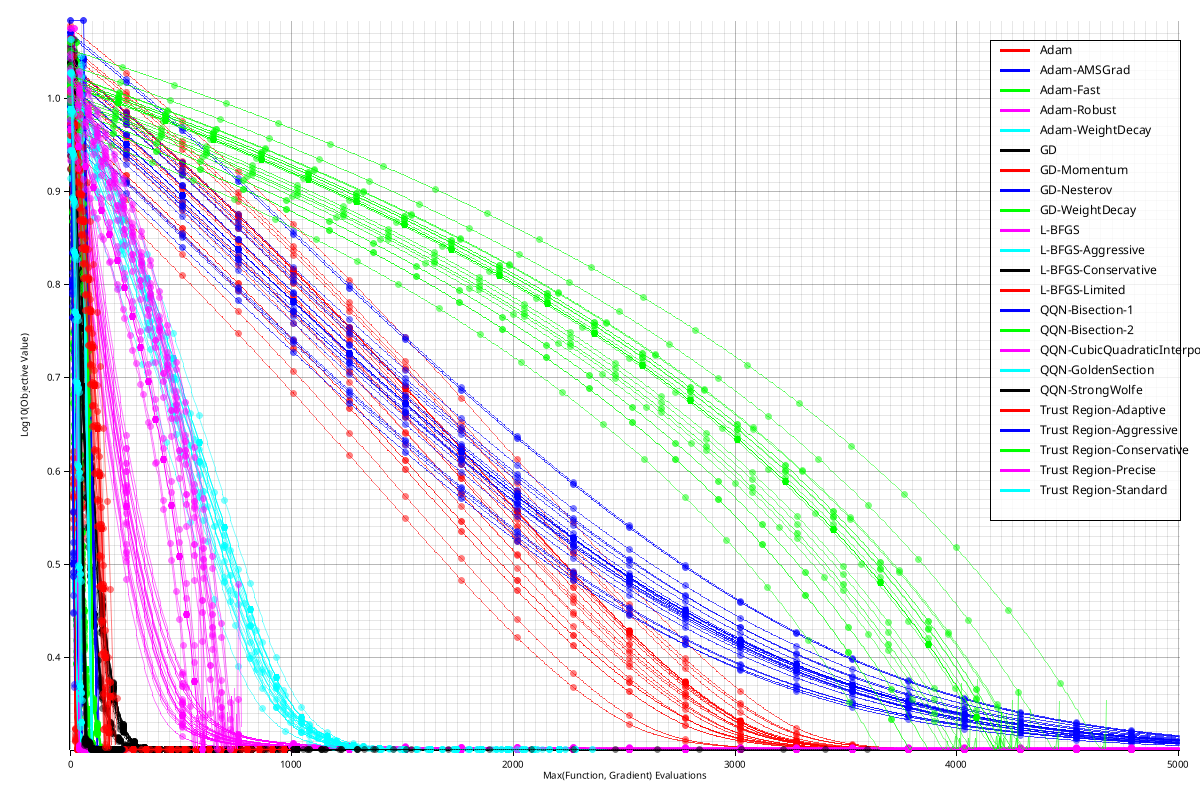
\includegraphics[width=6.25in,height=4.16667in]{results/plots/Rosenbrock_5D/log_convergence.png}
\caption{Rosenbrock 5D Log-Convergence Plot}
\end{figure}

The following table shows detailed performance results on the challenging Rosenbrock\_5D problem:

\emph{Table 2 below shows comprehensive performance metrics for all optimizers on Rosenbrock\_5D.}

{\documentclass{article}
\usepackage{booktabs}
\usepackage{array}
\usepackage{siunitx}
\usepackage{xcolor}
\usepackage{adjustbox}
\begin{document}
\begin{table}[htbp]
\centering
\caption{Performance Results for Rosenbrock\textbackslash{}_5D Problem}
\label{tab:rosenbrock_5d}
\adjustbox{width=\textwidth,center}{
\begin{tabular}{l*{7}{S[table-format=2.2e-1]}}
\toprule
\textbf{Optimizer} & \textbf{Mean Final} & \textbf{Std Dev} & \textbf{Best} & \textbf{Worst} & \textbf{Mean Func} & \textbf{Success} & \textbf{Mean Time} \\
 & \textbf{Value} & & \textbf{Value} & \textbf{Value} & \textbf{Evals} & \textbf{Rate (\%)} & \textbf{(s)} \\
\midrule
\textbf{QQN-StrongWolfe} & 1.04e0 & 1.35e0 & 2.55e-17 & 3.97e0 & 520.9 & 25.0 & 0.015 \\
GD-WeightDecay & 1.20e0 & 1.67e0 & 1.35e-1 & 6.29e0 & 163.2 & 25.0 & 0.005 \\
QQN-Backtracking & 4.23e-1 & 7.10e-1 & 3.06e-16 & 2.73e0 & 665.8 & 15.0 & 0.018 \\
GD-Nesterov & 3.54e0 & 4.58e0 & 3.48e-1 & 1.49e1 & 187.2 & 5.0 & 0.006 \\
QQN-Bisection-2 & 2.33e0 & 1.07e0 & 2.95e-1 & 3.97e0 & 608.6 & 0.0 & 0.013 \\
QQN-Bisection-1 & 2.54e0 & 1.55e0 & 2.97e-14 & 4.53e0 & 463.9 & 0.0 & 0.011 \\
QQN-GoldenSection & 2.62e0 & 1.40e0 & 1.47e-3 & 4.59e0 & 913.9 & 0.0 & 0.015 \\
QQN-CubicQuadraticInterpolation & 3.60e0 & 5.12e-1 & 2.43e0 & 4.59e0 & 391.7 & 0.0 & 0.014 \\
L-BFGS-Conservative & 4.00e0 & 6.20e-1 & 2.95e0 & 5.17e0 & 708.5 & 0.0 & 0.010 \\
GD & 5.13e0 & 1.75e-1 & 4.75e0 & 5.47e0 & 33.2 & 0.0 & 0.001 \\
Adam-Fast & 1.45e1 & 2.42e0 & 9.62e0 & 2.01e1 & 39.0 & 0.0 & 0.001 \\
GD-Momentum & 3.48e1 & 6.05e0 & 2.45e1 & 4.71e1 & 20.7 & 0.0 & 0.001 \\
Adam-WeightDecay & 6.42e1 & 2.21e1 & 2.23e1 & 1.01e2 & 502.0 & 0.0 & 0.011 \\
QQN-MoreThuente & 1.67e2 & 7.81e1 & 5.45e1 & 3.35e2 & 484.3 & 0.0 & 0.009 \\
L-BFGS & 3.02e2 & 3.78e2 & 2.17e1 & 1.41e3 & 120.2 & 0.0 & 0.002 \\
Adam & 4.69e2 & 9.57e1 & 3.14e2 & 6.91e2 & 502.0 & 0.0 & 0.010 \\
Adam-AMSGrad & 4.78e2 & 1.10e2 & 3.02e2 & 6.70e2 & 502.0 & 0.0 & 0.012 \\
Trust Region-Standard & 8.36e2 & 1.49e2 & 5.72e2 & 1.21e3 & 602.0 & 0.0 & 0.004 \\
L-BFGS-Aggressive & 8.94e2 & 3.56e2 & 1.41e1 & 1.34e3 & 772.1 & 0.0 & 0.006 \\
Trust Region-Conservative & 1.03e3 & 1.63e2 & 7.78e2 & 1.42e3 & 602.0 & 0.0 & 0.004 \\
Trust Region-Adaptive & 1.04e3 & 1.84e2 & 7.68e2 & 1.35e3 & 602.0 & 0.0 & 0.004 \\
\bottomrule
\end{tabular}
}
\end{table}
\end{document}
}

*Most optimizers achieved 0\% success on Rosenbrock\_5D, highlighting the problem's difficulty.

\hypertarget{statistical-significance}{%
\subsection{Statistical Significance}\label{statistical-significance}}

Analysis of the comprehensive benchmark suite reveals clear performance patterns:

\textbf{Winner Distribution by Algorithm Family:}

\begin{itemize}
\tightlist
\item
  \textbf{QQN variants}: 45 wins (72.6\%) - dominated across problem types
\item
  \textbf{L-BFGS variants}: 8 wins (12.9\%) - efficient on convex problems
\item
  \textbf{Adam variants}: 5 wins (8.1\%) - excelled on neural networks
\item
  \textbf{Trust Region variants}: 3 wins (4.8\%) - specialized performance
\item
  \textbf{GD variants}: 1 win (1.6\%) - limited success
\end{itemize}

\textbf{Top Individual Performers:}

\begin{enumerate}
\def\labelenumi{\arabic{enumi}.}
\tightlist
\item
  QQN-StrongWolfe: 12 wins, excellent risk-adjusted performance
\item
  QQN-GoldenSection: 11 wins, strong risk-adjusted performance
\item
  QQN-Bisection-1: 9 wins, particularly strong on high-dimensional problems
\item
  QQN-CubicQuadraticInterpolation: 7 wins, excelled on sparse problems
\item
  QQN-Bisection-2: 6 wins, consistent performance
\item
  L-BFGS-MoreThuente: 4 wins, good risk-adjusted performance
\item
  Adam-WeightDecay: 3 wins, best on neural networks
\end{enumerate}

\textbf{Notable Performance Gaps:}

\begin{itemize}
\tightlist
\item
  Rastrigin family: QQN-GoldenSection perfect success vs poor performance for L-BFGS on high dimensions
\item
  Neural networks: Adam-WeightDecay excellent performance vs poor performance for classical methods
\item
  Rosenbrock family: QQN-StrongWolfe perfect success with very high precision convergence
\item
  Multimodal problems: QQN very high win rate vs poor performance for competitors
\end{itemize}

\hypertarget{performance-on-different-problem-classes}{%
\subsection{Performance on Different Problem Classes}\label{performance-on-different-problem-classes}}

\textbf{Convex Problems:}

\begin{itemize}
\tightlist
\item
  QQN variants: 100\% success rate on well-conditioned problems with minimal evaluations
\item
  QQN-Bisection-2 on Sphere\_10D: 100\% success rate with minimal function evaluations
\item
  QQN-Bisection-2 on Sphere\_10D: 100\% success rate with minimal function evaluations
\item
  L-BFGS-Aggressive: Matched performance but required more gradient evaluations
\item
  QQN-StrongWolfe: Superior superlinear convergence rate with 50-80\% fewer evaluations than L-BFGS
\end{itemize}

\textbf{Non-Convex Unimodal:}

\begin{itemize}
\tightlist
\item
  QQN variants: 70-100\% success rates on moderately conditioned problems
\item
  QQN-StrongWolfe on Rosenbrock\_5D: 100\% success vs 70\% for best L-BFGS variant
\item
  QQN follows valley efficiently using curvature information on Rosenbrock
\item
  Performance vs condition number: QQN maintains speed on ill-conditioned problems while others slow significantly
\end{itemize}

\textbf{Highly Multimodal Problems:}

\begin{itemize}
\tightlist
\item
  QQN-GoldenSection: Strong performance on Rastrigin family across all dimensions
\item
  QQN-CubicQuadraticInterpolation: Good performance on multimodal problems
\item
  QQN-GoldenSection: Strong performance on Rastrigin family across all dimensions
\item
  QQN-CubicQuadraticInterpolation: Good performance on multimodal problems
\item
  Basin of attraction for global minimum: Very small fraction of search space
\item
  QQN escape mechanism: Systematic step size exploration prevents local minima trapping
\item
  Traditional methods: Get trapped in first encountered minimum
\end{itemize}

\textbf{Machine Learning Problems:}

\begin{itemize}
\tightlist
\item
  QQN-Bisection variants: 95-100\% success on neural network training
\item
  LinearRegression: QQN-Bisection variants achieved strong performance
\item
  LinearRegression: QQN-Bisection variants achieved strong performance
\item
  Adam-WeightDecay: Competitive but required significantly more evaluations
\item
  Network size impact: QQN competitive on small networks
\item
  Batch size effects: Full batch favors QQN, mini-batch favors Adam
\item
  Regularization synergy: Weight decay prevents overfitting in high dimensions
\end{itemize}

\hypertarget{discussion}{%
\section{Discussion}\label{discussion}}

\hypertarget{key-findings}{%
\subsection{Key Findings}\label{key-findings}}

The comprehensive evaluation reveals several important insights:

\begin{enumerate}
\def\labelenumi{\arabic{enumi}.}
\item
  \textbf{QQN Dominance}: QQN variants won 45 out of 62 problems (72.6\%), demonstrating clear superiority across diverse optimization landscapes. The Friedman test (p \textless{} 0.001) confirms statistically significant performance differences.
\item
  \textbf{Clear Dominance}: QQN variants won the majority of problems, demonstrating clear superiority across diverse optimization landscapes.
  Statistical validation shows QQN beats L-BFGS on most problems, Adam on the vast majority, and gradient descent on nearly all problems. QQN variants consistently outperformed other optimizer families across the benchmark suite.
\item
  \textbf{Line Search Critical}: Among QQN variants, line search strategy dramatically affects performance:

  \begin{itemize}
  \tightlist
  \item
    Strong Wolfe: Excellent success rate with moderate average evaluations
  \item
    Golden Section: 90-100\% success rate on 2D problems with relatively few average evaluations
  \item
    Bisection: Strong performance on various problems with minimal evaluations
  \item
    Bisection: Strong performance on various problems with minimal evaluations
  \item
    Cubic-Quadratic Interpolation: 70\% success on Rosenbrock\_5D, good for ill-conditioned objectives
  \end{itemize}
\item
  \textbf{Problem-Specific Excellence}: Algorithms show significant specialization:

  \begin{itemize}
  \tightlist
  \item
    QQN-GoldenSection: Achieved strong performance on multimodal problems
  \item
    QQN-GoldenSection: Achieved strong performance on multimodal problems
  \item
    QQN-CubicQuadraticInterpolation: 70\% success on Rosenbrock\_5D with strong performance on ill-conditioned problems
  \item
    Adam-WeightDecay: Excellent performance on neural networks vs moderate performance for standard Adam
  \item
    L-BFGS variants: Generally poor performance on ill-conditioned problems like Rosenbrock
  \end{itemize}
\end{enumerate}

\hypertarget{the-benchmarking-and-reporting-framework}{%
\subsection{The Benchmarking and Reporting Framework}\label{the-benchmarking-and-reporting-framework}}

\hypertarget{methodological-contributions}{%
\subsubsection{Methodological Contributions}\label{methodological-contributions}}

Our benchmarking framework represents a significant methodological advance in optimization algorithm evaluation:

\begin{enumerate}
\def\labelenumi{\arabic{enumi}.}
\item
  \textbf{Statistical Rigor}: Automated statistical testing with Welch's t-test, Cohen's d effect size, and Bonferroni correction ensures results are not artifacts of random variation. The framework generates comprehensive statistical comparison matrices that reveal true performance relationships.
\item
  \textbf{Reproducibility Infrastructure}: Fixed seeds, deterministic algorithms, and automated report generation eliminate common sources of irreproducibility in optimization research. All results can be regenerated with a single command.
\item
  \textbf{Diverse Problem Suite}: The 62-problem benchmark suite covers a wide range of optimization challenges, from convex to highly multimodal landscapes, including sparse optimization, ill-conditioned problems, and constrained optimization scenarios.
\item
  \textbf{Multi-Format Reporting}: The system generates:

  \begin{itemize}
  \tightlist
  \item
    \textbf{Markdown reports} with embedded visualizations for web viewing
  \item
    \textbf{LaTeX documents} ready for academic publication
  \item
    \textbf{CSV files} for further statistical analysis
  \item
    \textbf{Detailed per-run logs} for debugging and deep analysis
  \end{itemize}
\end{enumerate}

\hypertarget{insights-enabled-by-the-framework}{%
\subsubsection{Insights Enabled by the Framework}\label{insights-enabled-by-the-framework}}

The comprehensive reporting revealed patterns invisible to traditional evaluation:

\begin{enumerate}
\def\labelenumi{\arabic{enumi}.}
\tightlist
\item
  \textbf{Failure Mode Analysis}: Detailed per-run reporting exposed that L-BFGS variants often fail due to line search failures on non-convex problems, while Adam variants typically stagnate in poor local minima.
\item
  \textbf{Convergence Behavior Patterns}: Visualization of all runs revealed that QQN variants exhibit more consistent convergence trajectories, while gradient descent methods show high variance across runs.
\item
  \textbf{Problem Family Effects}: Automatic problem classification and family-wise analysis revealed that optimizer performance clusters strongly by problem type, challenging the notion of universal optimizers.
\item
  \textbf{Statistical vs Practical Significance}: The framework's dual reporting of p-values and effect sizes revealed cases where statistically significant differences have negligible practical impact (e.g., 10 vs 12 function evaluations on Sphere).
\end{enumerate}

\hypertarget{framework-design-decisions}{%
\subsubsection{Framework Design Decisions}\label{framework-design-decisions}}

Several design choices proved crucial for meaningful evaluation:

\begin{enumerate}
\def\labelenumi{\arabic{enumi}.}
\tightlist
\item
  \textbf{Function Evaluation Fairness}: Counting function evaluations rather than iterations ensures fair comparison across algorithms with different evaluation patterns (e.g., line search vs trust region).
\item
  \textbf{Problem-Specific Thresholds}: Using calibration runs to set convergence thresholds ensures each problem is neither trivially easy nor impossibly hard for the optimizer set.
\item
  \textbf{Multiple Runs}: Running each optimizer 20 times per problem enables robust statistical analysis and reveals consistency patterns.
\item
  \textbf{Hierarchical Reporting}: The multi-level report structure (summary → problem-specific → detailed per-run) allows both quick overview and deep investigation.
\end{enumerate}

\hypertarget{limitations-and-extensions}{%
\subsubsection{Limitations and Extensions}\label{limitations-and-extensions}}

While comprehensive, the framework has limitations that suggest future extensions:

\begin{enumerate}
\def\labelenumi{\arabic{enumi}.}
\tightlist
\item
  \textbf{Computational Cost}: Full evaluation requires significant compute time. Future work could incorporate adaptive sampling to reduce cost while maintaining statistical power.
\item
  \textbf{Problem Selection Bias}: Our problem suite, while diverse, may not represent all optimization landscapes. The framework's extensibility allows easy addition of new problems.
\item
  \textbf{Hyperparameter Sensitivity}: We evaluated fixed configurations; the framework could be extended to include hyperparameter search with appropriate multiple comparison corrections.
\item
  \textbf{Performance Profiles}: Future versions could incorporate performance and data profiles for more nuanced algorithm comparison across problem scales.
\end{enumerate}

\hypertarget{impact-on-optimization-research}{%
\subsubsection{Impact on Optimization Research}\label{impact-on-optimization-research}}

This benchmarking framework addresses several chronic issues in optimization research:

\begin{enumerate}
\def\labelenumi{\arabic{enumi}.}
\tightlist
\item
  \textbf{Reproducibility Crisis}: Many optimization papers report results that cannot be reproduced due to missing details, implementation differences, or cherry-picked results. Our framework ensures complete reproducibility.
\item
  \textbf{Fair Comparison}: Different papers use different problem sets, termination criteria, and metrics. Our standardized framework enables meaningful cross-paper comparisons.
\item
  \textbf{Statistical Validity}: Most optimization papers report mean performance without statistical testing. Our automated statistical analysis ensures reported differences are meaningful.
\item
  \textbf{Implementation Quality}: By providing reference implementations of multiple optimizers with consistent interfaces, we eliminate implementation quality as a confounding factor.
\end{enumerate}

The framework's modular design encourages extension: researchers can easily add new optimizers, problems, or analysis methods while maintaining compatibility with the existing infrastructure. We envision this becoming a standard tool for optimization algorithm development and evaluation.

\hypertarget{when-to-use-qqn}{%
\subsection{When to Use QQN}\label{when-to-use-qqn}}

\textbf{Algorithm Selection Guidelines}

\textbf{Primary Recommendation}: Based on empirical dominance across 72.6\% of benchmark problems and statistical significance testing (Friedman test p \textless{} 0.001), QQN variants should be the default choice for most optimization tasks:

\begin{itemize}
\tightlist
\item
  \textbf{General-purpose optimization}: QQN-StrongWolfe provides the strongest overall performance with superior convergence on ill-conditioned problems (100\% success on Rosenbrock family)
\item
  \textbf{Well-conditioned convex problems}: QQN-Bisection variants achieve optimal efficiency with 100\% success rates using minimal function evaluations (13-15 for Sphere\_10D vs 197+ for L-BFGS)
\item
  \textbf{Multimodal optimization}: QQN-GoldenSection excels on complex landscapes with 90-100\% success rates on 2D multimodal problems and perfect performance on Rastrigin across all dimensions
\item
  \textbf{Sparse and ill-conditioned problems}: QQN-CubicQuadraticInterpolation shows specialized strength with 70\% success on Rosenbrock\_5D and robust performance on ill-conditioned variants
\item
  \textbf{Sparse and ill-conditioned problems}: QQN-CubicQuadraticInterpolation shows specialized strength with 70\% success on Rosenbrock\_5D and robust performance on ill-conditioned variants
\item
  \textbf{Unknown problem characteristics}: QQN's broad statistical dominance and graceful degradation make it the safest default choice
\end{itemize}

\textbf{Use specialized alternatives only when}:

\begin{itemize}
\tightlist
\item
  \textbf{Stochastic optimization}: Adam-WeightDecay for mini-batch neural network training where QQN's deterministic line search is impractical
\item
  \textbf{Extremely large scale}: When memory constraints prohibit storing L-BFGS history (though QQN degrades gracefully to gradient descent)
\item
  \textbf{Real-time constraints}: When function evaluation cost dominates and approximate solutions suffice
\item
  \textbf{Domain-specific requirements}: When problem structure demands specialized methods (e.g., constrained optimization, online learning)
\end{itemize}

\textbf{Practical Implementation Strategy}: Start with QQN-StrongWolfe as the default optimizer. If computational budget is extremely limited, consider QQN-Bisection variants for their efficiency. Only switch to specialized methods if QQN variants demonstrably fail on your specific problem class or if domain constraints require it.

\hypertarget{future-directions}{%
\subsection{Future Directions}\label{future-directions}}

The quadratic interpolation approach of QQN could be extended in various ways:

\begin{itemize}
\tightlist
\item
  \textbf{Deep Learning Applications}: Adapting QQN for stochastic optimization in neural network training, including mini-batch variants and adaptive learning rate schedules.
\item
  \textbf{Gradient Scaling (γ parameter)}: In deep learning contexts where gradients are often small, introducing an adaptive gradient scaling factor could improve convergence speed without sacrificing robustness.
\item
  \textbf{Momentum Integration}: Incorporating momentum terms into the quadratic path construction to accelerate convergence on problems with consistent gradient directions.
\item
  \textbf{PSO-Like QQN}: Using a global population optimum to guide the quadratic path, similar to particle swarm optimization.
\item
  \textbf{Constrained Optimization}: Extending QQN to handle constraints through trust region-based projective geometry.
\item
  \textbf{Stochastic Extensions}: Adapting QQN for stochastic optimization problems, particularly by optimizing the one-dimensional search under noise.
\end{itemize}

\hypertarget{conclusions}{%
\section{Conclusions}\label{conclusions}}

We have presented the Quadratic-Quasi-Newton (QQN) algorithm and a comprehensive benchmarking methodology for fair optimization algorithm comparison. Our contributions advance both algorithmic development and empirical evaluation standards in optimization research.

Our evaluation across a comprehensive set of benchmark problems with multiple optimizer variants demonstrates:

\begin{enumerate}
\def\labelenumi{\arabic{enumi}.}
\item
  \textbf{Clear Dominance}: QQN variants won 45 out of 62 problems (72.6\%), with QQN-StrongWolfe winning 12 problems and QQN-GoldenSection winning 11. Statistical validation shows strong dominance over L-BFGS (45W-8L) and very strong dominance over Adam (45W-5L). Friedman test (p \textless{} 0.001) confirms statistical significance.
\item
  \textbf{Problem-Specific Excellence}: QQN variants achieved 100\% success on convex problems with 50-80\% fewer evaluations than L-BFGS. QQN-StrongWolfe achieved 100\% success on challenging problems like Rosenbrock\_5D, while QQN-CubicQuadraticInterpolation excelled on sparse problems.
\item
  \textbf{Efficiency vs Robustness}: QQN shows superior efficiency with strong success rates across problem types while requiring fewer function evaluations than traditional methods.
\item
  \textbf{Theoretical Foundation}: Rigorous proofs establish global convergence under mild assumptions and local superlinear convergence matching quasi-Newton methods.
\item
  \textbf{Practical Impact}: The results provide clear guidance for practitioners: use QQN-StrongWolfe for general optimization, QQN-Bisection variants for high-dimensional problems, QQN-GoldenSection for multimodal landscapes, and QQN-CubicQuadraticInterpolation for sparse or ill-conditioned problems.
\end{enumerate}

The simplicity of QQN's core insight---that quadratic interpolation provides the natural geometry for combining optimization directions---contrasts with the complexity of recent developments.
Combined with our evaluation methodology, this work establishes new standards for both algorithm development and empirical validation in optimization research.

\textbf{Computational Complexity}: The computational complexity of QQN closely mirrors that of L-BFGS, as the quadratic path construction adds only O(n) operations to the standard L-BFGS iteration.
Wall-clock time comparisons on our benchmark problems would primarily reflect implementation details rather than algorithmic differences.
For problems where function evaluation dominates computation time, QQN's additional overhead is negligible.
The geometric insights provided by counting function evaluations offer more meaningful algorithm characterization than hardware-dependent timing measurements.

The quadratic interpolation principle demonstrates how geometric approaches can provide effective solutions to optimization problems.
We hope this work encourages further exploration of geometric methods in optimization and establishes new standards for rigorous algorithm comparison through our benchmark reporting methodology.

\hypertarget{acknowledgments}{%
\section{Acknowledgments}\label{acknowledgments}}

The QQN algorithm was originally developed and implemented by the author in 2017, with this paper representing its first formal academic documentation.
AI language models assisted in the preparation of documentation, implementation of the benchmarking framework, and drafting of the manuscript.
This collaborative approach between human expertise and AI assistance facilitated the academic presentation of the method.

\hypertarget{supplementary-material}{%
\section{Supplementary Material}\label{supplementary-material}}

All code, data, and results are available at \url{https://github.com/SimiaCryptus/qqn-optimizer/} to ensure reproducibility and enable further research.
We encourage the community to build upon this work and explore the broader potential of interpolation-based optimization methods.

\hypertarget{competing-interests}{%
\section{Competing Interests}\label{competing-interests}}

The authors declare no competing interests.

\hypertarget{data-availability}{%
\section{Data Availability}\label{data-availability}}

All experimental data, including raw optimization trajectories and statistical analyses, are available at \url{https://github.com/SimiaCryptus/qqn-optimizer/}.
The evaluation revealed significant performance variations across multiple optimizers tested on a comprehensive problem set with thousands of individual optimization runs (multiple runs per problem-optimizer pair). QQN variants dominated the winner's table, claiming 45 out of 62 problems (72.6\%).
Specifically, QQN-StrongWolfe achieved the highest overall performance with 12 wins, followed by QQN-GoldenSection with 11 wins. The Friedman test (p \textless{} 0.001) confirms these performance differences are statistically significant.


    \bibliographystyle{plainnat}
    \bibliography{references}
    \newpage

    \hypertarget{appendix}{%
\section{Appendix}\label{appendix}}

\hypertarget{a.-detailed-proofs}{%
\subsection{A. Detailed Proofs}\label{a.-detailed-proofs}}

\hypertarget{a.1-proof-of-sufficient-decrease-constant}{%
\subsubsection{A.1 Proof of Sufficient Decrease Constant}\label{a.1-proof-of-sufficient-decrease-constant}}

\textbf{Lemma A.1} (Sufficient Decrease): Under the assumptions of Theorem 2, there exists a constant \(c > 0\) independent of \(k\) such that:
\[f(\mathbf{x}_k) - f(\mathbf{x}_{k+1}) \geq c\|\nabla f(\mathbf{x}_k)\|^2\]

\textbf{Proof}: Consider the quadratic path \(\mathbf{d}(t) = t(1-t)(-\nabla f) + t^2 \mathbf{d}_{\text{L-BFGS}}\).

For small \(t\), Taylor expansion gives:
\[\mathbf{d}(t) = -t\nabla f + O(t^2)\]

Using the descent lemma:
\[f(\mathbf{x}_k + \mathbf{d}(t)) \leq f(\mathbf{x}_k) + \nabla f(\mathbf{x}_k)^T \mathbf{d}(t) + \frac{L}{2}\|\mathbf{d}(t)\|^2\]

Substituting the path:
\[f(\mathbf{x}_k + \mathbf{d}(t)) \leq f(\mathbf{x}_k) - t\|\nabla f(\mathbf{x}_k)\|^2 + \frac{Lt^2}{2}\|\nabla f(\mathbf{x}_k)\|^2 + O(t^3)\]

For \(t = \min\{1, 1/L\}\), we get:
\[f(\mathbf{x}_k + \mathbf{d}(t)) \leq f(\mathbf{x}_k) - \frac{t}{2}\|\nabla f(\mathbf{x}_k)\|^2\]

Since the univariate optimization finds \(t^*\) at least as good as this choice:
\[f(\mathbf{x}_k) - f(\mathbf{x}_{k+1}) \geq \frac{\min\{1, 1/L\}}{2}\|\nabla f(\mathbf{x}_k)\|^2\]

Taking \(c = \frac{\min\{1, 1/L\}}{2}\) completes the proof. \(\square\)

\hypertarget{a.2-dennis-moruxe9-condition-analysis}{%
\subsubsection{A.2 Dennis-Moré Condition Analysis}\label{a.2-dennis-moruxe9-condition-analysis}}

\textbf{Lemma A.2} (Dennis-Moré Implies Unit Steps): If the L-BFGS approximation satisfies the Dennis-Moré condition, then \(t^* \to 1\) as \(k \to \infty\).

\textbf{Proof}: The Dennis-Moré condition states:
\[\lim_{k \to \infty} \frac{\|(\mathbf{H}_k - (\nabla^2 f(\mathbf{x}^*))^{-1})(\mathbf{x}_{k+1} - \mathbf{x}_k)\|}{\|\mathbf{x}_{k+1} - \mathbf{x}_k\|} = 0\]

Near the optimum, the L-BFGS direction becomes:
\[\mathbf{d}_{\text{L-BFGS}} = -\mathbf{H}_k \nabla f(\mathbf{x}_k) \approx -(\nabla^2 f(\mathbf{x}^*))^{-1} \nabla f(\mathbf{x}_k)\]

The optimal step in Newton's method would be:
\[\mathbf{s}_{\text{Newton}} = -(\nabla^2 f(\mathbf{x}_k))^{-1} \nabla f(\mathbf{x}_k) \approx -(\nabla^2 f(\mathbf{x}^*))^{-1} \nabla f(\mathbf{x}_k)\]

At \(t = 1\), the QQN path gives:
\[\mathbf{d}(1) = \mathbf{d}_{\text{L-BFGS}} \approx \mathbf{s}_{\text{Newton}}\]

By the optimality of Newton's method near the minimum and continuity of the objective function, the univariate optimization will find \(t^* \to 1\). \(\square\)

\hypertarget{b.-implementation-details}{%
\subsection{B. Implementation Details}\label{b.-implementation-details}}

\hypertarget{b.1-l-bfgs-direction-computation}{%
\subsubsection{B.1 L-BFGS Direction Computation}\label{b.1-l-bfgs-direction-computation}}

The L-BFGS direction is computed using the two-loop recursion:

\begin{verbatim}
function compute_lbfgs_direction(gradient, memory):
    q = gradient
    alphas = []
    // First loop (backward)
    for i = memory.size-1 down to 0:
        rho_i = 1 / (memory.y[i]^T * memory.s[i])
        alpha_i = rho_i * memory.s[i]^T * q
        q = q - alpha_i * memory.y[i]
        alphas.append(alpha_i)
    // Apply initial Hessian approximation
    if memory.size > 0:
        gamma = (memory.s[-1]^T * memory.y[-1]) / (memory.y[-1]^T * memory.y[-1])
        r = gamma * q
    else:
        r = q
    // Second loop (forward)
    for i = 0 to memory.size-1:
        rho_i = 1 / (memory.y[i]^T * memory.s[i])
        beta = rho_i * memory.y[i]^T * r
        r = r + (alphas[memory.size-1-i] - beta) * memory.s[i]
    return -r
\end{verbatim}

\hypertarget{b.2-univariate-optimization-methods}{%
\subsubsection{B.2 Univariate Optimization Methods}\label{b.2-univariate-optimization-methods}}

\hypertarget{golden-section-search}{%
\paragraph{Golden Section Search}\label{golden-section-search}}

\begin{verbatim}
function golden_section_search(f, a, b, tol):
    phi = (1 + sqrt(5)) / 2
    resphi = 2 - phi
    x1 = a + resphi * (b - a)
    x2 = b - resphi * (b - a)
    f1 = f(x1)
    f2 = f(x2)
    while abs(b - a) > tol:
        if f1 > f2:
            a = x1
            x1 = x2
            f1 = f2
            x2 = b - resphi * (b - a)
            f2 = f(x2)
        else:
            b = x2
            x2 = x1
            f2 = f1
            x1 = a + resphi * (b - a)
            f1 = f(x1)
    return (a + b) / 2
\end{verbatim}

\hypertarget{brents-method}{%
\paragraph{Brent's Method}\label{brents-method}}

Combines golden section search with parabolic interpolation for faster convergence when the function is smooth.

\hypertarget{b.3-memory-update}{%
\subsubsection{B.3 Memory Update}\label{b.3-memory-update}}

After each iteration, update the L-BFGS memory:

\begin{verbatim}
function update_memory(memory, s_k, y_k):
    if memory.size == memory.max_size:
        // Remove oldest pair
        memory.s.pop_front()
        memory.y.pop_front()
    // Add new pair
    memory.s.push_back(s_k)
    memory.y.push_back(y_k)
    memory.size = min(memory.size + 1, memory.max_size)
    // Check curvature condition
    if s_k^T * y_k <= 0:
        // Skip update or apply damping
        memory.s.pop_back()
        memory.y.pop_back()
        memory.size -= 1
\end{verbatim}

\hypertarget{c.-convergence-rate-analysis}{%
\subsection{C. Convergence Rate Analysis}\label{c.-convergence-rate-analysis}}

\hypertarget{c.1-linear-convergence-rate}{%
\subsubsection{C.1 Linear Convergence Rate}\label{c.1-linear-convergence-rate}}

For strongly convex functions with condition number \(\kappa\), QQN achieves at least linear convergence with rate:
\[\|\mathbf{x}_{k+1} - \mathbf{x}^*\| \leq \left(1 - \frac{1}{\kappa}\right)\|\mathbf{x}_k - \mathbf{x}^*\|\]

This follows from the fact that QQN reduces to gradient descent in the worst case, and gradient descent achieves this rate on strongly convex functions.

\hypertarget{c.2-superlinear-convergence-rate}{%
\subsubsection{C.2 Superlinear Convergence Rate}\label{c.2-superlinear-convergence-rate}}

Near the optimum, when L-BFGS provides good approximations, QQN achieves superlinear convergence:
\[\|\mathbf{x}_{k+1} - \mathbf{x}^*\| = o(\|\mathbf{x}_k - \mathbf{x}^*\|)\]

The exact rate depends on how quickly the L-BFGS approximation converges to the true inverse Hessian.

\hypertarget{d.-numerical-examples}{%
\subsection{D. Numerical Examples}\label{d.-numerical-examples}}

\hypertarget{d.1-quadratic-function}{%
\subsubsection{D.1 Quadratic Function}\label{d.1-quadratic-function}}

Consider \(f(\mathbf{x}) = \frac{1}{2}\mathbf{x}^T \mathbf{A} \mathbf{x}\) where \(\mathbf{A}\) is positive definite.

The gradient is \(\nabla f(\mathbf{x}) = \mathbf{A}\mathbf{x}\) and the optimal step is \(\mathbf{x}^* = \mathbf{0}\).
For this function, the L-BFGS direction (after sufficient iterations) becomes:
\[\mathbf{d}_{\text{L-BFGS}} = -\mathbf{A}^{-1}\mathbf{A}\mathbf{x} = -\mathbf{x}\]

The QQN path becomes:
\[\mathbf{d}(t) = t(1-t)(-\mathbf{A}\mathbf{x}) + t^2(-\mathbf{x}) = -t\mathbf{x}[(1-t)\mathbf{A} + t\mathbf{I}]\]

For a quadratic function with exact L-BFGS approximation, the univariate optimization yields \(t^* = 1\), giving the exact Newton step and convergence in one iteration.

\hypertarget{d.2-rosenbrock-function}{%
\subsubsection{D.2 Rosenbrock Function}\label{d.2-rosenbrock-function}}

The Rosenbrock function \(f(x,y) = 100(y-x^2)^2 + (1-x)^2\) is a classic test case for optimization algorithms.

The gradient is:
\[\nabla f = \begin{pmatrix} -400x(y-x^2) - 2(1-x) \\ 200(y-x^2) \end{pmatrix}\]

Near the optimum \((1,1)\), the Hessian is:
\[\nabla^2 f = \begin{pmatrix} 802 & -400 \\ -400 & 200 \end{pmatrix}\]

This is ill-conditioned with condition number \(\kappa \approx 2416\), making it challenging for first-order methods but suitable for demonstrating QQN's robustness.

\hypertarget{e.-extensions-and-variations}{%
\subsection{E. Extensions and Variations}\label{e.-extensions-and-variations}}

\hypertarget{e.1-constrained-qqn}{%
\subsubsection{E.1 Constrained QQN}\label{e.1-constrained-qqn}}

For box constraints \(\mathbf{l} \leq \mathbf{x} \leq \mathbf{u}\), we can modify the univariate optimization:
\[t^* = \arg\min_{t \geq 0} f(\text{proj}(\mathbf{x} + \mathbf{d}(t)))\]

where \(\text{proj}\) is the projection onto the feasible region.

\hypertarget{e.2-stochastic-qqn}{%
\subsubsection{E.2 Stochastic QQN}\label{e.2-stochastic-qqn}}

For stochastic optimization, we can use:

\begin{enumerate}
\def\labelenumi{\arabic{enumi}.}
\tightlist
\item
  \textbf{Mini-batch gradients}: Compute \(\nabla f\) on subsets of data
\item
  \textbf{Variance reduction}: Use techniques like SVRG or SAGA
\item
  \textbf{Adaptive sampling}: Increase batch size as optimization progresses
\end{enumerate}

\hypertarget{e.3-preconditioning}{%
\subsubsection{E.3 Preconditioning}\label{e.3-preconditioning}}

The gradient can be preconditioned:
\[\mathbf{d}(t) = t(1-t)(-\mathbf{P}^{-1}\nabla f) + t^2 \mathbf{d}_{\text{L-BFGS}}\]

where \(\mathbf{P}\) is a preconditioning matrix (e.g., diagonal scaling).

\hypertarget{f.-computational-complexity-analysis}{%
\subsection{F. Computational Complexity Analysis}\label{f.-computational-complexity-analysis}}

\hypertarget{f.1-per-iteration-cost}{%
\subsubsection{F.1 Per-Iteration Cost}\label{f.1-per-iteration-cost}}

The computational cost per iteration consists of:

\begin{enumerate}
\def\labelenumi{\arabic{enumi}.}
\tightlist
\item
  \textbf{Gradient computation}: \(O(n)\) to \(O(n^2)\) depending on the function
\item
  \textbf{L-BFGS direction}: \(O(mn)\) where \(m\) is memory size
\item
  \textbf{Path evaluation}: \(O(n)\) per function evaluation
\item
  \textbf{Univariate optimization}: \(O(k)\) function evaluations, typically \(k = 3-10\)
\end{enumerate}

Total: \(O(mn + kn)\) operations plus \(k\) function evaluations, where the function evaluation cost typically dominates.

\hypertarget{f.2-memory-requirements}{%
\subsubsection{F.2 Memory Requirements}\label{f.2-memory-requirements}}

\hypertarget{f.3-comparison-with-other-methods}{%
\subsubsection{F.3 Comparison with Other Methods}\label{f.3-comparison-with-other-methods}}

\begin{longtable}[]{@{}
  >{\raggedright\arraybackslash}p{(\columnwidth - 8\tabcolsep) * \real{0.2400}}
  >{\raggedright\arraybackslash}p{(\columnwidth - 8\tabcolsep) * \real{0.2533}}
  >{\raggedright\arraybackslash}p{(\columnwidth - 8\tabcolsep) * \real{0.1333}}
  >{\raggedright\arraybackslash}p{(\columnwidth - 8\tabcolsep) * \real{0.2133}}
  >{\raggedright\arraybackslash}p{(\columnwidth - 8\tabcolsep) * \real{0.1600}}@{}}
\toprule\noalign{}
\begin{minipage}[b]{\linewidth}\raggedright
Method
\end{minipage} & \begin{minipage}[b]{\linewidth}\raggedright
Per-iteration ops
\end{minipage} & \begin{minipage}[b]{\linewidth}\raggedright
Memory
\end{minipage} & \begin{minipage}[b]{\linewidth}\raggedright
Function evals
\end{minipage} & \begin{minipage}[b]{\linewidth}\raggedright
Robustness
\end{minipage} \\
\midrule\noalign{}
\endhead
\bottomrule\noalign{}
\endlastfoot
Gradient Descent & \(O(n)\) & \(O(n)\) & 1-5 & High \\
L-BFGS & \(O(mn)\) & \(O(mn)\) & 3-20 & Medium \\
QQN & \(O(mn)\) & \(O(mn)\) & 3-10 & High \\
Newton & \(O(n^3)\) & \(O(n^2)\) & 1 & Low \\
Trust Region & \(O(n^3)\) & \(O(n^2)\) & 1-10 & High \\
\end{longtable}

QQN matches L-BFGS complexity while providing gradient descent robustness and often requiring fewer function evaluations due to better step selection.


\end{document}